% E2: sentiment classification. Every number in this file comes from results/e2_sentiment.json
% (python experiments/e2_sentiment.py) or, for published systems, from the cited paper/table.

\subsection{E2: Sentiment classification}
\label{sec:e2}

\paragraph{Setup.}
We train multinomial Naive Bayes (NB), Rocchio and $k$NN (Section~\ref{sec:methodology}) on the
official SentiMix Hinglish training split (14{,}000 tweets) under each of the four normalisation
modes (\texttt{raw}, \texttt{soundex}, \texttt{hkey}, \texttt{hkey\_clusters}); the variant clusters
used by \texttt{hkey\_clusters} are learned from the training split only. The H-Key settings were
fixed on the E1 dev groups before this experiment was run: \texttt{hkey} uses the V-norm vowel
policy, and \texttt{hkey\_clusters} merges words that share a V-drop key with trigram cosine
$\theta=0.85$. As an ablation we also run \texttt{hkey\_vdrop}, H-Key with the V-drop vowel policy,
which E1 found to have much higher recall. It was added after the settings were frozen, is reported
separately, and was not used to choose any setting. NB uses term counts;
Rocchio and $k$NN use ltc tf-idf vectors. The only hyperparameter, $k$ for $k$NN, is chosen on the
dev split (3{,}000 tweets) by macro $F_1$. We first searched the values used in the lecture,
$k\in\{1,3,9,15\}$; the best value was $k=15$ in every mode, the edge of that grid, so we extended
the search to $\{21,31,45,61\}$. The final choice is $k=61$ in every mode. Dev $F_1$ was still
rising slowly at $k=61$ (for \texttt{raw}: 56.5 at $k=15$, 59.5 at $k=45$, 60.1 at $k=61$); larger
values were not explored. The test split (3{,}000 tweets) is predicted once per configuration.

\paragraph{Metrics.}
Our main metric is the macro-averaged $F_1$ over the three classes,
$F_1^{\text{macro}}=\frac{1}{3}\sum_{c} F_{1,c}$ with $F_{1,c}=\frac{2P_cR_c}{P_c+R_c}$, which weights
every class equally. The official SemEval-2020 Task~9 metric is different: \citet{patwa2020semeval}
(Section~3.1) ``use weighted F1 score on the test data'', where ``the F1 scores are calculated for
each class and then their average is weighted by support (number of true instances for each class)'',
i.e.\ $F_1^{\text{weighted}}=\sum_c \frac{n_c}{N}F_{1,c}$. We therefore report both, and use
\emph{weighted} $F_1$ for every comparison with published systems.

To decide whether a difference between two modes is more than noise we use a paired bootstrap
test: we draw 1{,}000 test sets of 3{,}000 tweets with replacement from the test split (seed 42),
score both systems on each resampled set, and report the 95\% percentile interval of the
difference in macro $F_1$ together with the one-sided $p$-value, the fraction of resamples in which
the normalised system is not better than \texttt{raw}.

\begin{table}[t]
\centering
\small
\caption{E2 results on the SentiMix Hinglish test set (\%). $\Delta$ = change in test macro $F_1$
relative to \texttt{raw} for the same classifier (significance in Table~\ref{tab:e2-boot}). Dev
$F_1$ is macro $F_1$ on the dev split. $^\dagger$\,Ablation (H-Key with V-drop), not one of the
four main modes.}
\label{tab:e2-main}
\begin{tabular}{llrrrrrrrr}
\toprule
 & Mode & $k$ & Dev $F_1$ & Macro $P$ & Macro $R$ & Macro $F_1$ & $\Delta$ & Weighted $F_1$ & Acc. \\
\midrule
NB      & \texttt{raw}            & --  & 57.9 & 63.5 & 65.4 & 63.4 & --   & 62.7 & 64.1 \\
        & \texttt{soundex}        & --  & 54.9 & 60.3 & 61.9 & 60.5 & $-3.0$ & 59.8 & 60.8 \\
        & \texttt{hkey}           & --  & 57.6 & 63.2 & 65.1 & 63.0 & $-0.4$ & 62.3 & 63.8 \\
        & \texttt{hkey\_clusters} & --  & 57.6 & 63.3 & 65.2 & 63.1 & $-0.3$ & 62.4 & 63.9 \\
        & \texttt{hkey\_vdrop}$^\dagger$ & -- & 57.8 & 62.7 & 64.5 & 62.6 & $-0.8$ & 61.9 & 63.2 \\
\midrule
Rocchio & \texttt{raw}            & --  & 53.9 & 60.4 & 62.3 & 59.6 & --   & 58.8 & 60.7 \\
        & \texttt{soundex}        & --  & 54.7 & 60.4 & 61.5 & 60.7 & $+1.1$ & 60.2 & 60.6 \\
        & \texttt{hkey}           & --  & 54.5 & 60.9 & 62.8 & 60.4 & $+0.8$ & 59.6 & 61.3 \\
        & \texttt{hkey\_clusters} & --  & 54.9 & 60.9 & 62.8 & 60.4 & $+0.8$ & 59.6 & 61.4 \\
        & \texttt{hkey\_vdrop}$^\dagger$ & -- & 55.9 & 62.0 & 63.4 & 62.2 & $+2.6$ & 61.7 & 62.5 \\
\midrule
$k$NN   & \texttt{raw}            & 61  & 60.1 & 65.8 & 65.4 & 65.4 & --   & 65.0 & 65.2 \\
        & \texttt{soundex}        & 61  & 56.3 & 60.6 & 60.1 & 60.3 & $-5.1$ & 60.0 & 59.9 \\
        & \texttt{hkey}           & 61  & 59.5 & 65.2 & 65.2 & 65.0 & $-0.5$ & 64.6 & 64.9 \\
        & \texttt{hkey\_clusters} & 61  & 59.6 & 64.7 & 64.8 & 64.5 & $-0.9$ & 64.1 & 64.5 \\
        & \texttt{hkey\_vdrop}$^\dagger$ & 61 & 57.6 & 64.1 & 64.2 & 64.1 & $-1.3$ & 63.7 & 63.9 \\
\midrule
\multicolumn{3}{l}{Majority class (\emph{neutral})} & -- & -- & -- & 17.9 & -- & 19.7 & 36.7 \\
\bottomrule
\end{tabular}
\end{table}

\begin{table}[t]
\centering
\small
\caption{Paired bootstrap test of the change in test macro $F_1$ (percentage points) of each
normalised mode relative to \texttt{raw}, same classifier. 1{,}000 resamples; $p$ is one-sided
(fraction of resamples with $\Delta\le 0$); $p<0.001$ means no resample had $\Delta\le 0$. The
12 tests are not corrected for multiple comparisons. $^\dagger$\,Ablation.}
\label{tab:e2-boot}
\begin{tabular}{llrrr}
\toprule
 & Mode & $\Delta$ macro $F_1$ & 95\% interval & $p$ \\
\midrule
NB      & \texttt{soundex}        & $-3.00$ & $[-4.74,\ -1.31]$ & 1.000 \\
        & \texttt{hkey}           & $-0.41$ & $[-1.31,\ +0.49]$ & 0.800 \\
        & \texttt{hkey\_clusters} & $-0.30$ & $[-1.27,\ +0.61]$ & 0.731 \\
        & \texttt{hkey\_vdrop}$^\dagger$ & $-0.84$ & $[-2.20,\ +0.55]$ & 0.866 \\
\midrule
Rocchio & \texttt{soundex}        & $+1.09$ & $[-0.42,\ +2.82]$ & 0.098 \\
        & \texttt{hkey}           & $+0.81$ & $[+0.04,\ +1.57]$ & 0.019 \\
        & \texttt{hkey\_clusters} & $+0.79$ & $[+0.08,\ +1.55]$ & 0.018 \\
        & \texttt{hkey\_vdrop}$^\dagger$ & $+2.65$ & $[+1.17,\ +4.13]$ & $<0.001$ \\
\midrule
$k$NN   & \texttt{soundex}        & $-5.12$ & $[-7.05,\ -3.28]$ & 1.000 \\
        & \texttt{hkey}           & $-0.47$ & $[-1.71,\ +0.73]$ & 0.761 \\
        & \texttt{hkey\_clusters} & $-0.89$ & $[-2.20,\ +0.40]$ & 0.930 \\
        & \texttt{hkey\_vdrop}$^\dagger$ & $-1.34$ & $[-3.12,\ +0.26]$ & 0.943 \\
\bottomrule
\end{tabular}
\end{table}

\begin{figure}[t]
\centering
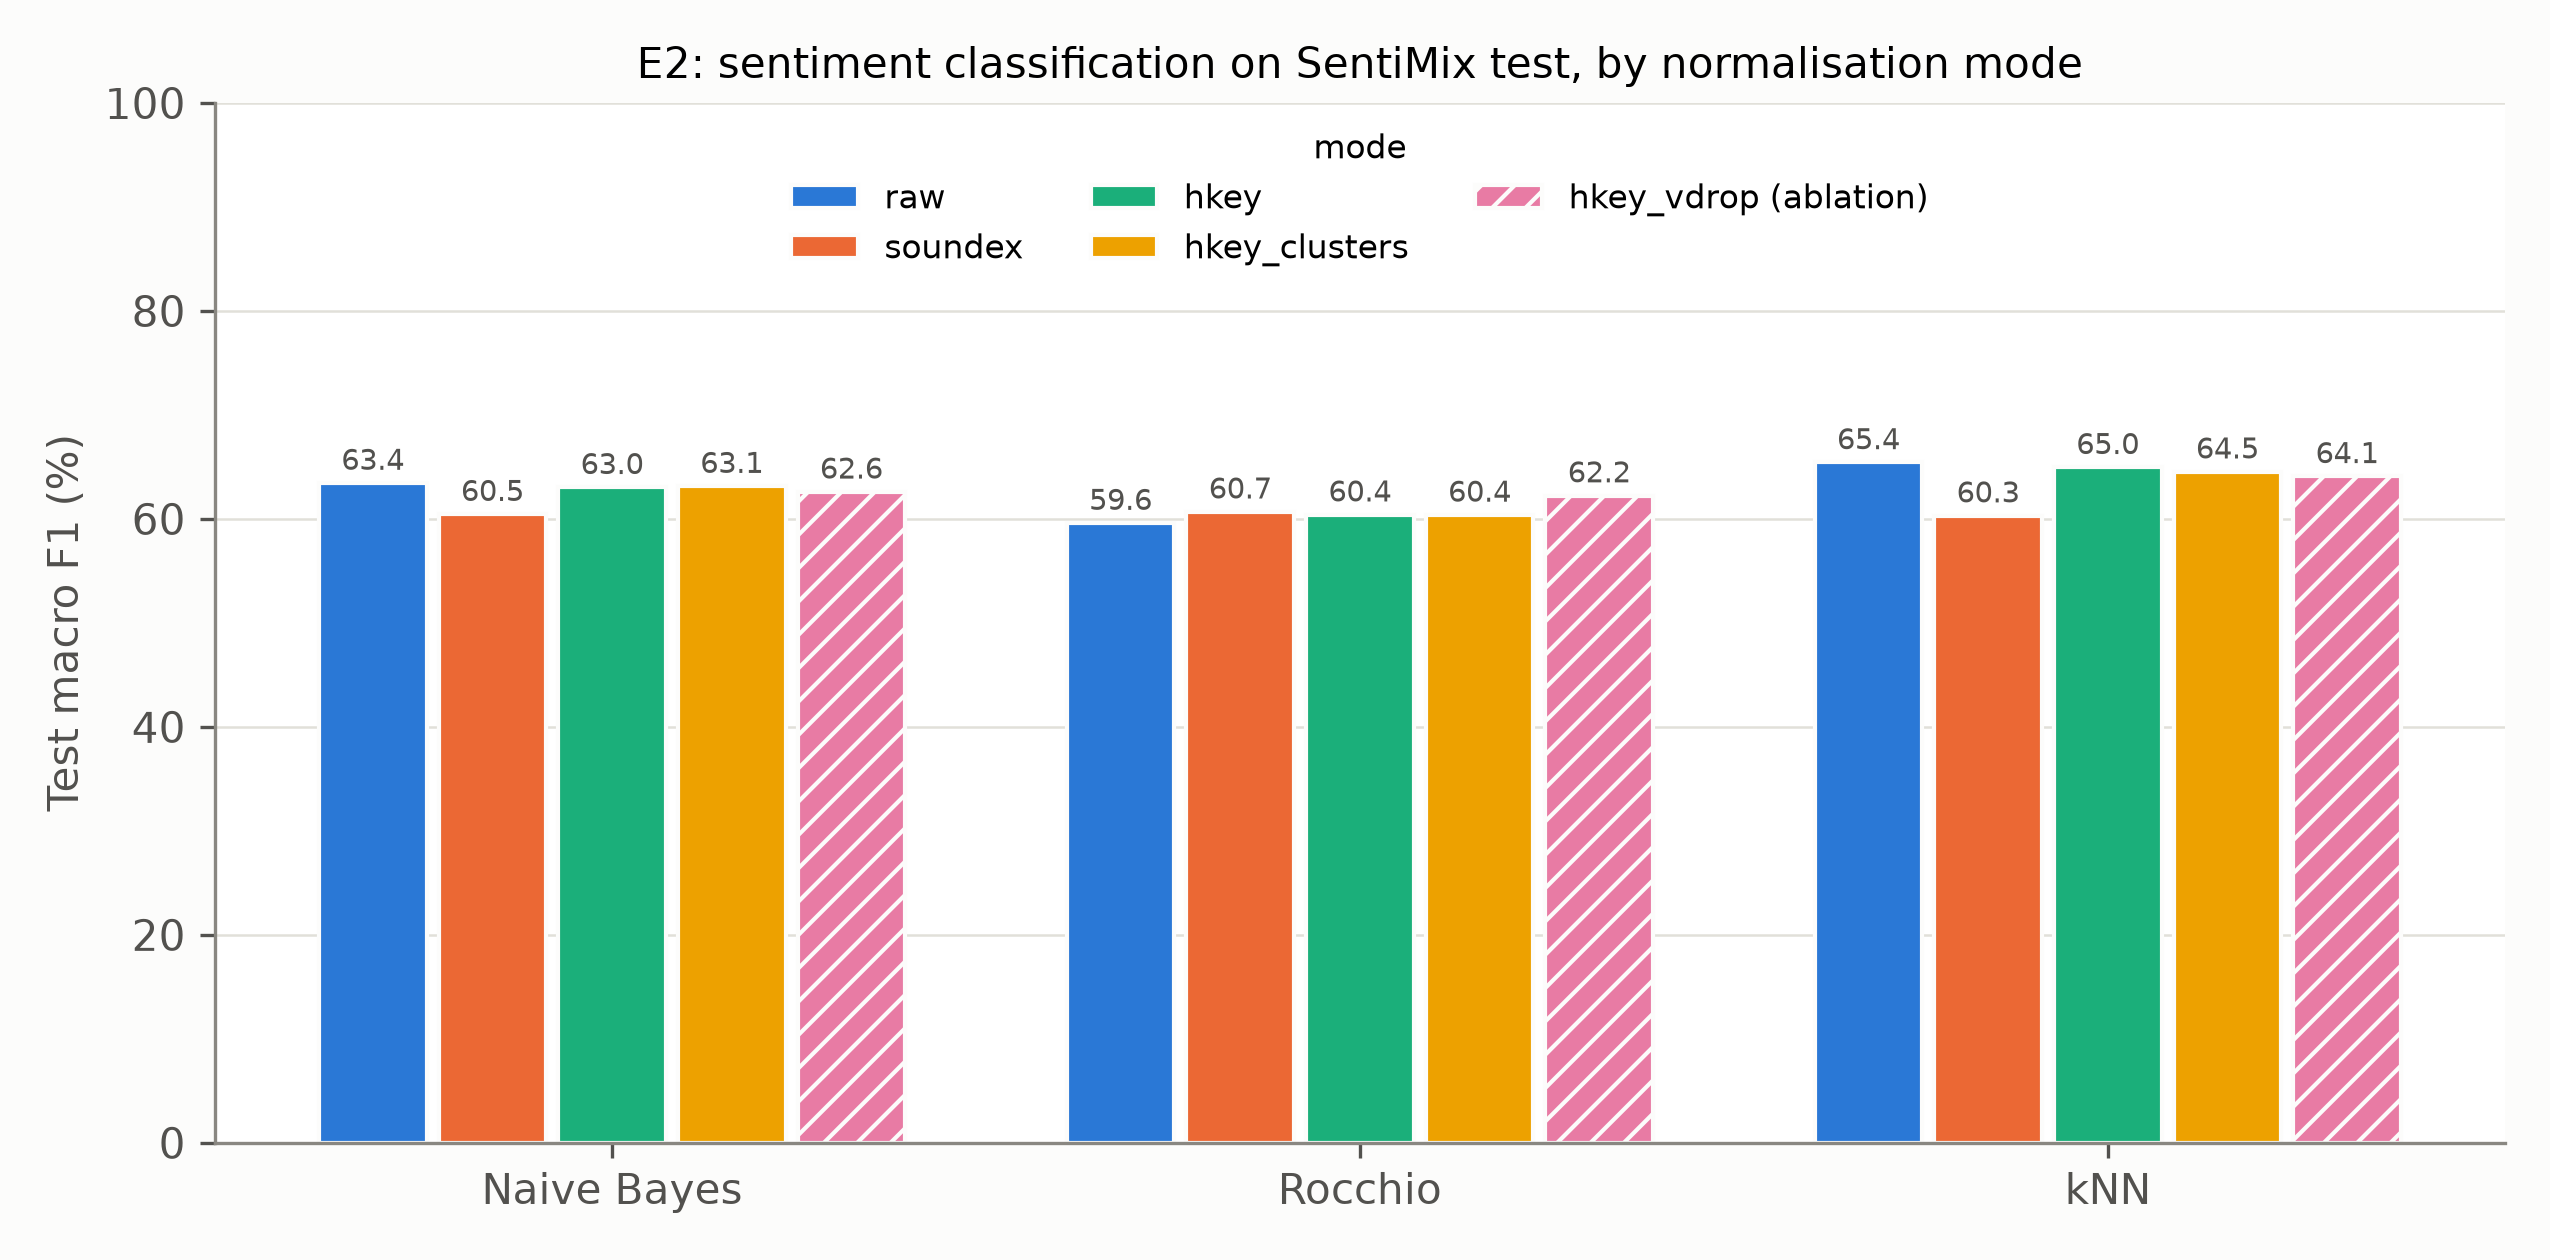
\includegraphics[width=\linewidth]{../figures/e2_f1_bar.png}
\caption{Test macro $F_1$ for each classifier and normalisation mode (values from
Table~\ref{tab:e2-main}). Hatched bars: the \texttt{hkey\_vdrop} ablation.}
\label{fig:e2-bar}
\end{figure}

\paragraph{Effect of normalisation.}
Table~\ref{tab:e2-main} and Figure~\ref{fig:e2-bar} give the results and Table~\ref{tab:e2-boot}
their significance. Normalisation shrinks the training vocabulary from 30{,}265 types
(\texttt{raw}) to 25{,}208 (\texttt{hkey}), 25{,}132 (\texttt{hkey\_clusters}), 13{,}037
(\texttt{hkey\_vdrop}) and 4{,}249 (\texttt{soundex}). Its effect on classification depends on the
classifier:
\begin{itemize}
\item \textbf{Rocchio} is the only classifier that gains significantly, and the gain is small:
$+0.81$ macro $F_1$ with \texttt{hkey} (95\% interval $[+0.04, +1.57]$, $p=0.019$) and $+0.79$ with
\texttt{hkey\_clusters} ($[+0.08, +1.55]$, $p=0.018$). Both intervals lie only just above zero.
The gain also appears on dev ($+0.6$ and $+1.0$). A plausible explanation is that its centroids
are averages over sparse vectors, and merging spellings concentrates the weight of a word that was
spread over several variants.
\item \textbf{$k$NN} does not gain. With $k=61$, \texttt{hkey} and \texttt{hkey\_clusters} score
0.5 and 0.9 points below \texttt{raw} on test (both intervals include zero) and 0.5 below on dev.
\item \textbf{NB} does not gain either: $-0.4$ and $-0.3$, both within noise. Possible reasons are
that add-one smoothing already lets NB use rare spellings as separate evidence, and that any merge
of two words with different sentiment costs NB directly.
\item \textbf{Lecture Soundex} significantly hurts NB ($-3.0$) and $k$NN ($-5.1$). It reduces
30{,}265 word types to 4{,}249 four-character codes, so many unrelated words share a feature.
\item \textbf{The V-drop ablation} merges more aggressively than the main H-Key modes (13{,}037
types, a 56.9\% cut) and gives Rocchio a larger gain: $+2.65$ ($[+1.17, +4.13]$, $p<0.001$; $+2.0$
on dev). For NB ($-0.84$) and $k$NN ($-1.34$) the change is within noise. Since the 12 tests in
Table~\ref{tab:e2-boot} are not corrected for multiple comparisons, we note that with a Bonferroni
correction (threshold $0.05/12\approx0.004$ on the one-sided $p$) the only gain that remains
significant is Rocchio's with V-drop; Rocchio's $+0.8$ with the main H-Key modes ($p\approx0.02$)
would not survive it.
\end{itemize}
In short, the phonetic equivalence classes cut the vocabulary by about a sixth (16.7\% for
\texttt{hkey}, 17.0\% for \texttt{hkey\_clusters}) without a significant loss for any classifier,
and with a small significant gain for Rocchio; lecture Soundex, which merges far more aggressively,
does significant harm. The ablation shows a trade-off: V-drop, which E1 found to group variants with
higher recall but lower precision, helps Rocchio more than the frozen V-norm setting, but not NB or
$k$NN. Normalisation does not make any classifier better than the best
unnormalised one: the best single system on test is $k$NN on \texttt{raw} (65.4 macro $F_1$).

\begin{table}[t]
\centering
\small
\caption{Per-class test $F_1$ (\%). $^\dagger$\,Ablation.}
\label{tab:e2-perclass}
\begin{tabular}{llrrr}
\toprule
 & Mode & Negative & Neutral & Positive \\
\midrule
NB      & \texttt{raw}            & 69.3 & 47.3 & 73.7 \\
        & \texttt{soundex}        & 65.3 & 46.1 & 69.9 \\
        & \texttt{hkey}           & 69.2 & 46.7 & 73.3 \\
        & \texttt{hkey\_clusters} & 69.0 & 46.8 & 73.6 \\
        & \texttt{hkey\_vdrop}$^\dagger$ & 68.9 & 46.8 & 72.1 \\
\midrule
Rocchio & \texttt{raw}            & 66.2 & 41.6 & 71.0 \\
        & \texttt{soundex}        & 64.4 & 48.9 & 68.7 \\
        & \texttt{hkey}           & 66.5 & 43.1 & 71.6 \\
        & \texttt{hkey\_clusters} & 66.5 & 42.9 & 71.7 \\
        & \texttt{hkey\_vdrop}$^\dagger$ & 65.9 & 48.8 & 72.1 \\
\midrule
$k$NN   & \texttt{raw}            & 67.6 & 56.0 & 72.7 \\
        & \texttt{soundex}        & 61.7 & 53.0 & 66.3 \\
        & \texttt{hkey}           & 66.9 & 54.9 & 73.1 \\
        & \texttt{hkey\_clusters} & 66.8 & 54.2 & 72.7 \\
        & \texttt{hkey\_vdrop}$^\dagger$ & 65.7 & 54.6 & 72.0 \\
\bottomrule
\end{tabular}
\end{table}

\begin{figure}[t]
\centering
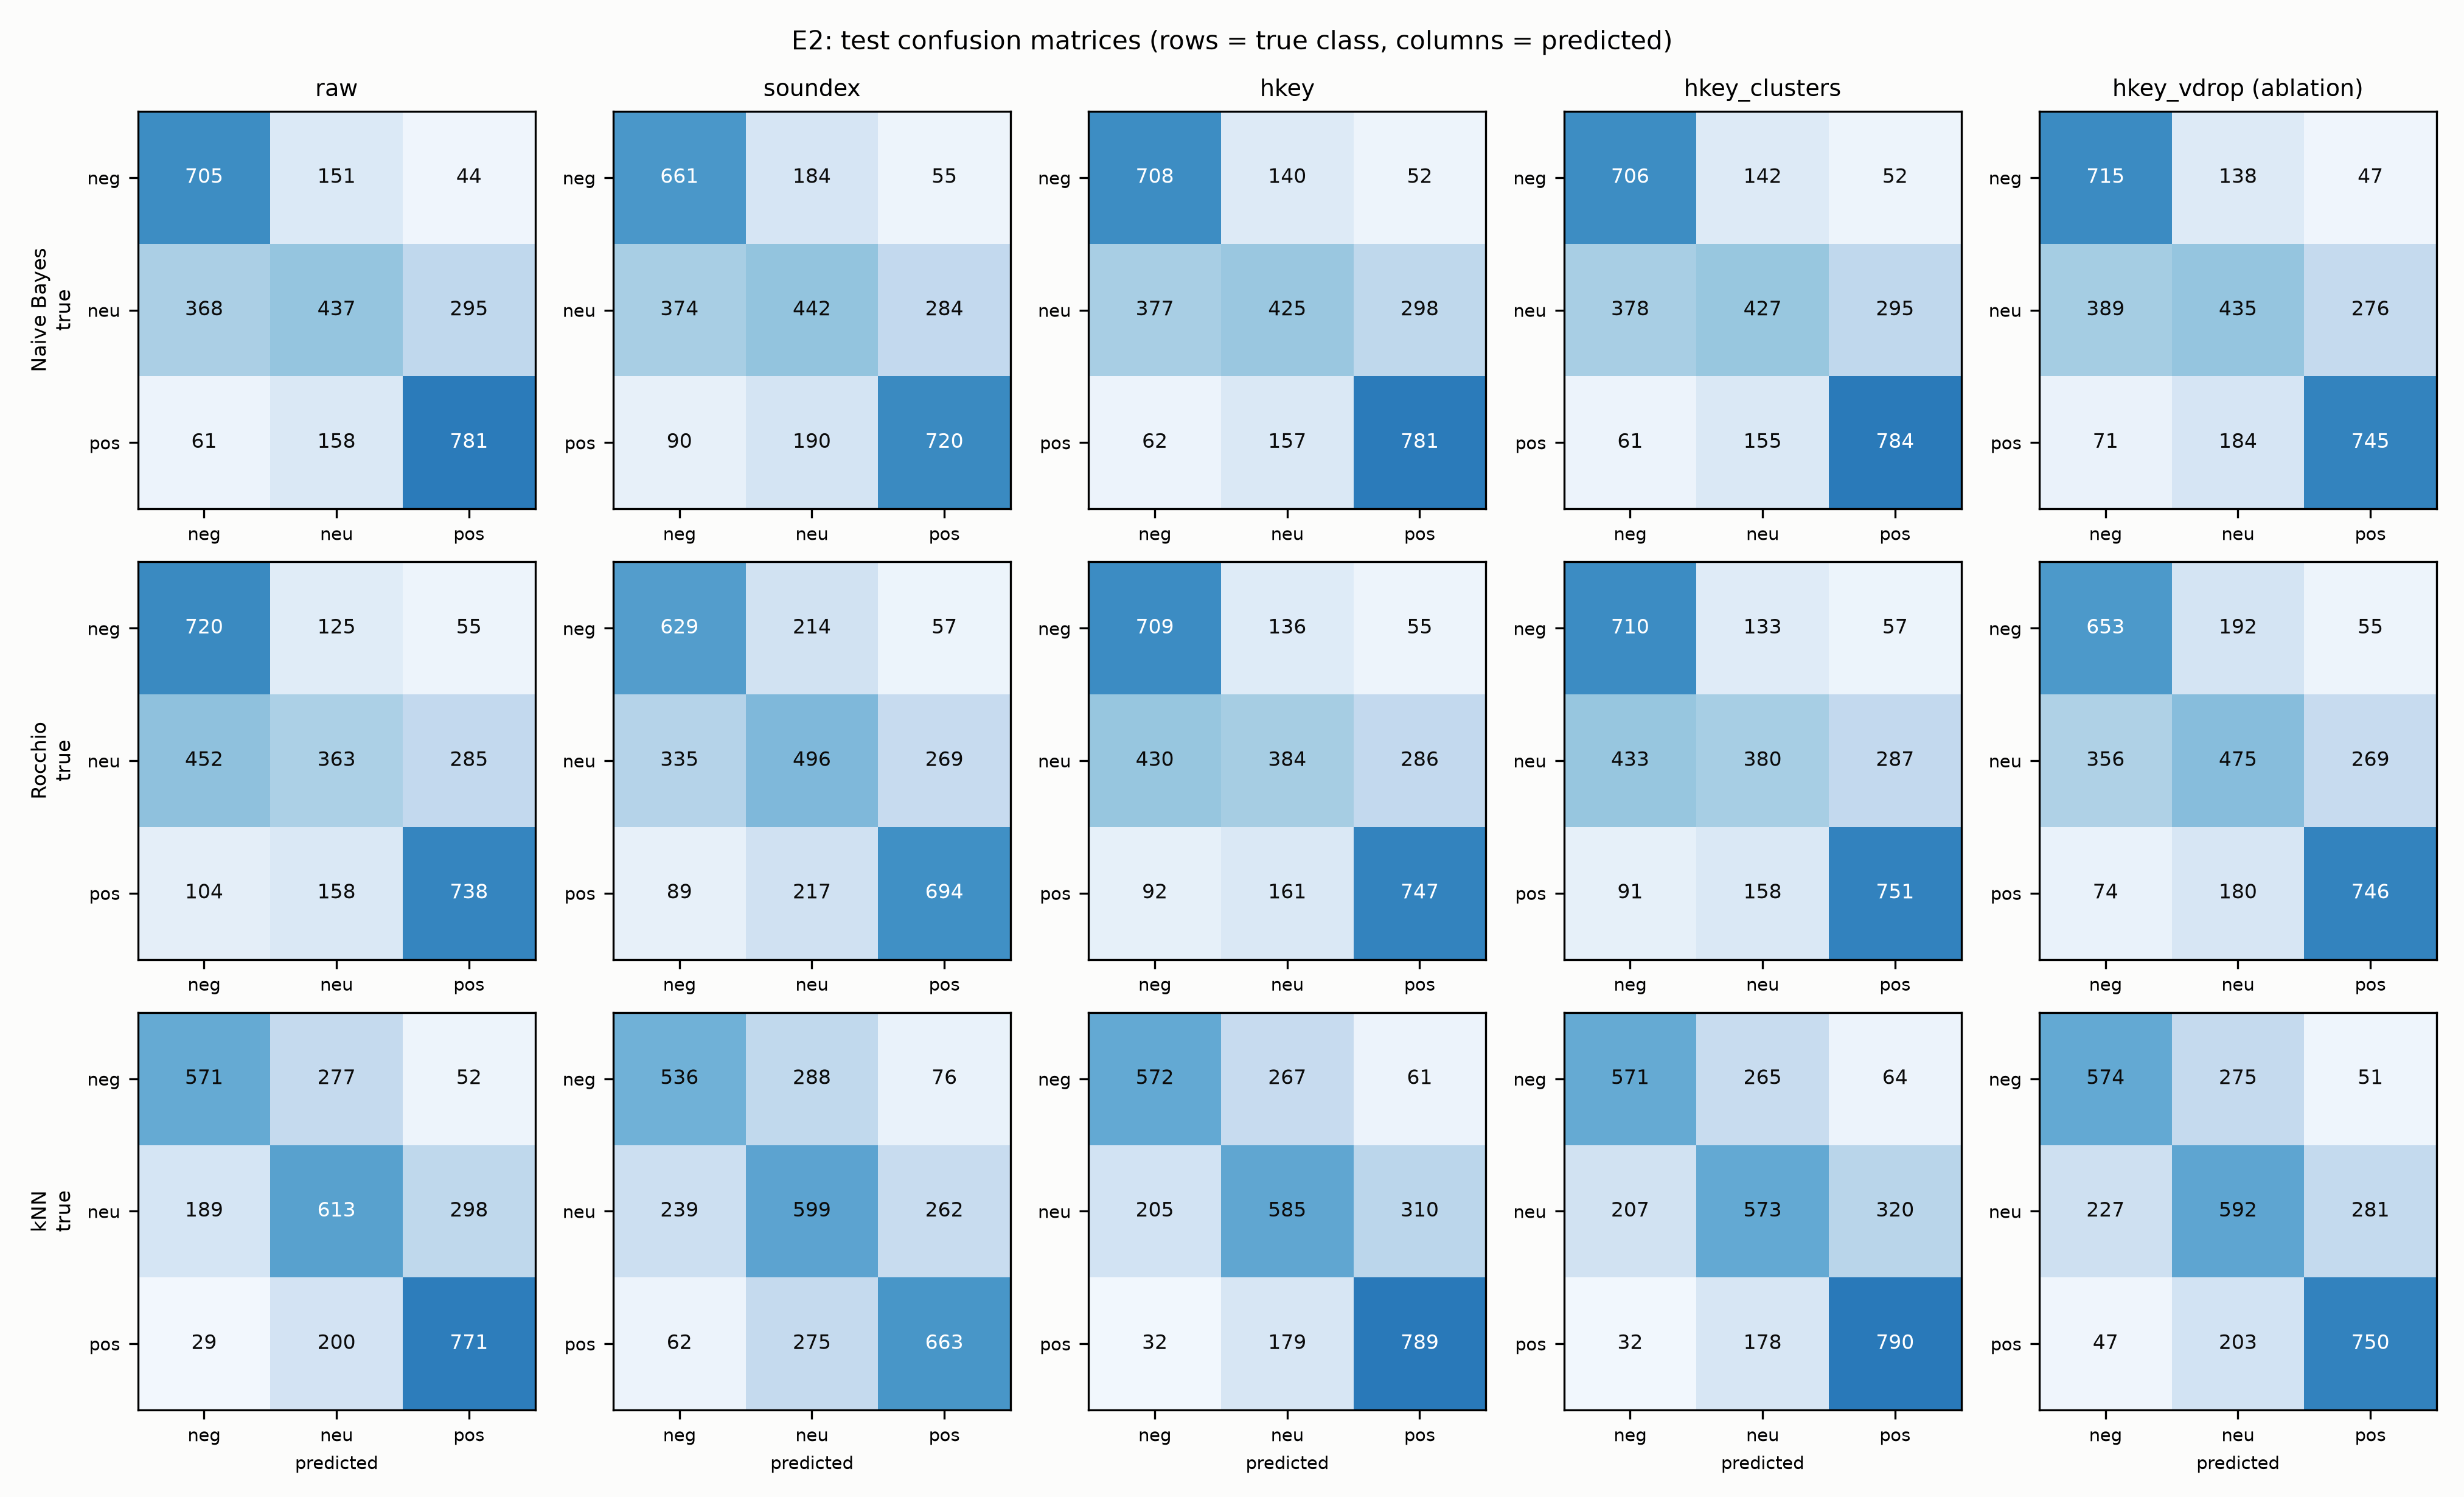
\includegraphics[width=\linewidth]{../figures/e2_confusion.png}
\caption{Test confusion matrices (rows: true class; columns: predicted class).}
\label{fig:e2-confusion}
\end{figure}

\paragraph{Per-class behaviour.}
Neutral is the hardest class for every system (Table~\ref{tab:e2-perclass}), as it is for the
published systems (Table~\ref{tab:e2-compare}). The confusion matrices (Figure~\ref{fig:e2-confusion})
show why: neutral tweets are misclassified in both directions, while negative and positive are rarely
confused with each other. Rocchio on \texttt{raw} sends 452 of the 1{,}100 neutral test tweets to the
negative centroid; with \texttt{hkey} this falls to 430 and neutral $F_1$ rises from 41.6 to 43.1,
the largest per-class change behind Rocchio's gain. The V-drop ablation goes further: 356
neutral tweets go to the negative centroid and neutral $F_1$ reaches 48.8. A single centroid is a poor model of a class such as
neutral, which mixes news, advertisements and anything that is neither positive nor negative
\citep{patwa2020semeval}. $k$NN, which decides from the local neighbourhood instead of one
centroid, has the best neutral $F_1$ of our classifiers (56.0 on \texttt{raw}).

\paragraph{Why accuracy is reported but not used.}
On this dataset accuracy and macro $F_1$ are close (e.g.\ NB \texttt{raw}: 64.1 vs.\ 63.4), because
the Hinglish classes are roughly balanced (36.7\% of test tweets are neutral). Accuracy rewards a
system for the majority class: a classifier that always answers \emph{neutral} already scores
36.7\% accuracy while its macro $F_1$ is 17.9, since it never finds a negative or positive tweet.
On a skewed collection the gap becomes extreme. In the Spanglish part of the same task 80.8\% of test
tweets are positive \citep[Table~1]{patwa2020semeval}, so the same trivial classifier would reach
80.8\% accuracy. Precision, recall and $F_1$ per class expose this; accuracy does not.

\paragraph{Comparison with published systems.}
Table~\ref{tab:e2-compare} compares our systems with SemEval-2020 Task~9 Hinglish results, all in
weighted $F_1$ on the same official test split. For each classifier we show \texttt{raw} and the
main normalised mode with the best \emph{dev} macro $F_1$, so the selection does not use the test set
(the ablation is not a candidate).

\begin{table}[t]
\centering
\small
\caption{Comparison with published SemEval-2020 Task~9 Hinglish systems (test set, \%). All
$F_1$ values are the task's official weighted $F_1$ and its per-class $F_1$. Published rows are
copied from \citet[Table~3]{patwa2020semeval}.}
\label{tab:e2-compare}
\begin{tabular}{lrrrr}
\toprule
System & Weighted $F_1$ & Neg.\ $F_1$ & Neu.\ $F_1$ & Pos.\ $F_1$ \\
\midrule
KK2018, rank 1 (XLM-R) \citep{patwa2020semeval}                         & 75.0 & 76.9 & 68.9 & 79.9 \\
Reed, rank 4 (bagged BERT-large) \citep{gopalan2020reed}                & 71.3 & 73.0 & 64.3 & 77.5 \\
Organisers' M-BERT baseline, rank 45 \citep{patwa2020semeval}           & 65.4 & 68.3 & 58.1 & 70.7 \\
\midrule
Ours: $k$NN ($k=61$), \texttt{raw}                                      & 65.0 & 67.6 & 56.0 & 72.7 \\
Ours: $k$NN ($k=61$), \texttt{hkey\_clusters}                           & 64.1 & 66.8 & 54.2 & 72.7 \\
Ours: NB, \texttt{raw}                                                  & 62.7 & 69.3 & 47.3 & 73.7 \\
Ours: NB, \texttt{hkey}                                                 & 62.3 & 69.2 & 46.7 & 73.3 \\
Ours: Rocchio, \texttt{raw}                                             & 58.8 & 66.2 & 41.6 & 71.0 \\
Ours: Rocchio, \texttt{hkey\_clusters}                                  & 59.6 & 66.5 & 42.9 & 71.7 \\
Majority class (\emph{neutral})                                         & 19.7 &  0.0 & 53.7 &  0.0 \\
\bottomrule
\end{tabular}
\end{table}

Our classical models are clearly below the best systems. The strongest, $k$NN on \texttt{raw}
(65.0 weighted $F_1$), is 10.0 points below the winning system (75.0) and 6.3 points below
\citet{gopalan2020reed} (71.3). It is 0.4 points below the organisers' multilingual BERT baseline
(65.4), which 44 of the 61 Hinglish teams beat \citep{patwa2020semeval}; we cannot test whether
this small difference is significant because the baseline's predictions are not available. Per
class, $k$NN on \texttt{raw} is 0.7 points below the baseline on negative (67.6 vs.\ 68.3), 2.1
below on neutral (56.0 vs.\ 58.1) and 2.0 above on positive (72.7 vs.\ 70.7). We make no claim to
be competitive with the top systems; the remaining gap to them is largest on the neutral class.

A second comparison is possible on the dev split, because \citet{gopalan2020reed} report dev
accuracy for their models. They found that fine-tuning BERT gave 62.2\% (\texttt{bert-base-cased})
and at best 63.9\% dev accuracy (63.8\% in their Section~6), and that a two-layer feed-forward
network on bag-of-words (unigram and bigram) features reached 60.0\%, which led them to conclude
that BERT's success here ``is probably not due to a deep understanding of the code-mixed
language''. Our $k$NN on \texttt{raw} reaches 59.9\% dev accuracy, 0.1 points below their
bag-of-words network and 2.3 below fine-tuned \texttt{bert-base-cased}; NB on \texttt{raw}, which
has no tuned hyperparameter, reaches 58.6\%. The $k$NN figure is slightly optimistic because $k$
was chosen on dev, as their figures are, since they also tuned on the validation set
\citep{gopalan2020reed}. These systems use no neural network, no pre-training and no GPU. The
entire E2 run (feature extraction, variant clustering, training, the $k$ search, evaluation of all
15 configurations including the ablation, and the bootstrap tests) takes 21.9 seconds on a CPU; training NB on the 14{,}000
training tweets takes 0.04 s, and $k$NN classifies the 3{,}000 test tweets in 0.3 s.
